\documentclass[tikz,border=2mm]{standalone}

\usepackage{amsmath}
\usetikzlibrary{arrows,positioning}
\usetikzlibrary{fit,backgrounds}
\usepackage{xcolor}

\begin{document}

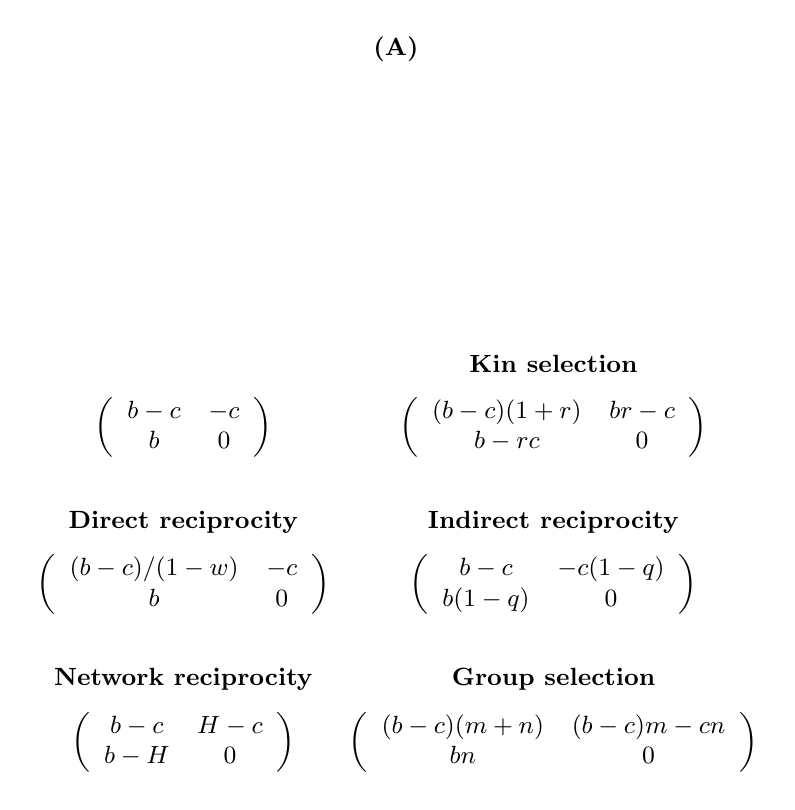
\begin{tikzpicture}[
    >=stealth,
    font=\small,
    gamelabel/.style={
        font=\scriptsize,
        align=center,
        text width=1.75cm,
        inner sep=2pt
    },
    reglabel/.style={
        font=\scriptsize,
        align=center,
        text width=1.75cm,
        inner sep=0pt
    }
]

% ---------------------------------
% Colors
% ---------------------------------
\colorlet{pdcol}{red!12}
\colorlet{hdcol}{green!14}
\colorlet{shcol}{blue!10}
\colorlet{hmcol}{orange!12}

% ---------------------------------
% Left: payoff matrix
% ---------------------------------
\node at (0, 5) {\textbf{(A)}};

\node at (-2.7, 0.2) {
    $\left(
    \begin{array}{cc}
    b-c & -c \\
    b & 0
    \end{array}
    \right)$
};

\node at (2, 1) {\textbf{Kin selection}};

\node at (2, 0.2) {
    $\left(
    \begin{array}{cc}
    (b-c)(1+r) & br -c \\
    b - rc & 0
    \end{array}
    \right)$
};

\node at (-2.7, 1-2) {\textbf{Direct reciprocity}};

\node at (-2.7, 0.2-2) {
    $\left(
    \begin{array}{cc}
    (b-c)/(1-w) & -c \\
    b & 0
    \end{array}
    \right)$
};

\node at (2, 1-2) {\textbf{Indirect reciprocity}};

\node at (2, 0.2-2) {
    $\left(
    \begin{array}{cc}
    b-c & -c(1-q) \\
    b(1-q) & 0
    \end{array}
    \right)$
};

\node at (-2.7, 1-2-2) {\textbf{Network reciprocity}};

\node at (-2.7, 0.2-2-2) {
    $\left(
    \begin{array}{cc}
    b-c & H-c \\
    b-H & 0
    \end{array}
    \right)$
};

\node at (2, 1-2-2) {\textbf{Group selection}};

\node at (2, 0.2-2-2) {
    $\left(
    \begin{array}{cc}
    (b-c)(m+n) & (b-c)m - cn \\
    bn & 0
    \end{array}
    \right)$
};

\end{tikzpicture}
\end{document}